\documentclass[border=1cm]{standalone}
\usepackage{tikz}
\usetikzlibrary{math}
\begin{document}
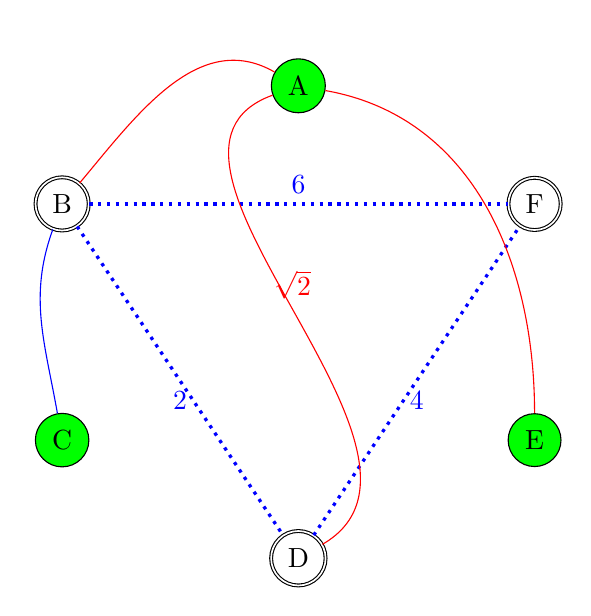
\begin{tikzpicture}[scale=3]
\node[circle,draw, double] (b) at (0,0) {B};
\node[circle,draw, double] (f) at (2,0) {F};
\node[circle,draw, double] (d) at (1,-1.5) {D};
\draw[blue,dotted,very thick] (b) to node[midway, above]{6} (f);
\draw[blue,dotted,very thick] (b) to node[midway, below]{2}(d);
\draw[blue,dotted,very thick] (d) to node[midway, below]{4}(f);
\node[circle,draw,fill=green] (c) at (0,-1) {C};
\node[circle,draw,fill=green] (a) at (1,0.5) {A};
\node[circle,draw,fill=green] (e) at (2,-1) {E};
\draw[blue] (b) to[out=250, in=100] (c);
\draw[red] (b) to[out=50, in=150] (a);
\draw[red] (a) to[out=200, in=30] node[midway, above]{$\sqrt{2}$} (d);
\draw[red] (a) to[out=350, in=90] (e);
\end{tikzpicture}

\begin{tikzpicture}[scale=2]
% Draw the x and y axis, label the axes and the origin
\draw[gray, ->] (-1.2,0) -- (1.6,0) node[right]{$x$} node[pos=0.53, below]{$O$};
\draw[gray, ->] (0,-1.2) -- (0,3.9) node[above]{$y$};
\draw[fill,gray] (0,0) circle [radius=1pt];



% Plot the curve
\draw[blue, thick] [domain=-1:1.5, samples=150] plot (\x, {exp(\x)})
node[right]{$y=e^x$};
\draw[black, thick, domain=0.3:1.6, samples=200] plot (\x, {ln(\x)})
node[right]{$y=\ln(x)$};
% Note: the r in the argument of the cosine signifies that we enter \x in radians
% Mark x=1 on x-axis
\fill[gray] (1,0) circle (0.03);
\node[gray, below] at (1,0) {$x=1$};
% Mark y=1 on y-axis
\fill[gray] (0,1) circle (0.03);
\node[gray, left] at (0,1) {$y=1$};

\end{tikzpicture}


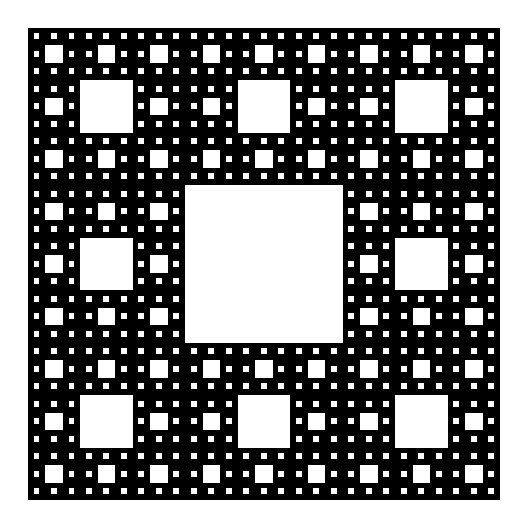
\begin{tikzpicture}
\def\S{6}
\def\D{4}
\tikzmath{
function carpet(\x,\y,\s,\d){
if (\d==0) then {
{ \fill (\x,\y) rectangle ++(\s,\s); };
} else {
\ns=\s/3;
carpet(\x,\y,\ns,\d-1);
carpet(\x+\ns,\y,\ns,\d-1);
carpet(\x+2*\ns,\y,\ns,\d-1);
carpet(\x,\y+\ns,\ns,\d-1);
carpet(\x+2*\ns,\y+\ns,\ns,\d-1);
carpet(\x,\y+2*\ns,\ns,\d-1);
carpet(\x+\ns,\y+2*\ns,\ns,\d-1);
carpet(\x+2*\ns,\y+2*\ns,\ns,\d-1);
};
};
carpet(0,0,\S,\D);
}
\end{tikzpicture}


\end{document}
